\documentclass[1p]{elsarticle_modified}
%\bibliographystyle{elsarticle-num}

%\usepackage[colorlinks]{hyperref}
%\usepackage{abbrmath_seonhwa} %\Abb, \Ascr, \Acal ,\Abf, \Afrak
\usepackage{amsfonts}
\usepackage{amssymb}
\usepackage{amsmath}
\usepackage{amsthm}
\usepackage{scalefnt}
\usepackage{amsbsy}
\usepackage{kotex}
\usepackage{caption}
\usepackage{subfig}
\usepackage{color}
\usepackage{graphicx}
\usepackage{xcolor} %% white, black, red, green, blue, cyan, magenta, yellow
\usepackage{float}
\usepackage{setspace}
\usepackage{hyperref}

\usepackage{tikz}
\usetikzlibrary{arrows}

\usepackage{multirow}
\usepackage{array} % fixed length table
\usepackage{hhline}

%%%%%%%%%%%%%%%%%%%%%
\makeatletter
\renewcommand*\env@matrix[1][\arraystretch]{%
	\edef\arraystretch{#1}%
	\hskip -\arraycolsep
	\let\@ifnextchar\new@ifnextchar
	\array{*\c@MaxMatrixCols c}}
\makeatother %https://tex.stackexchange.com/questions/14071/how-can-i-increase-the-line-spacing-in-a-matrix
%%%%%%%%%%%%%%%

\usepackage[normalem]{ulem}

\newcommand{\msout}[1]{\ifmmode\text{\sout{\ensuremath{#1}}}\else\sout{#1}\fi}
%SOURCE: \msout is \stkout macro in https://tex.stackexchange.com/questions/20609/strikeout-in-math-mode

\newcommand{\cancel}[1]{
	\ifmmode
	{\color{red}\msout{#1}}
	\else
	{\color{red}\sout{#1}}
	\fi
}

\newcommand{\add}[1]{
	{\color{blue}\uwave{#1}}
}

\newcommand{\replace}[2]{
	\ifmmode
	{\color{red}\msout{#1}}{\color{blue}\uwave{#2}}
	\else
	{\color{red}\sout{#1}}{\color{blue}\uwave{#2}}
	\fi
}

\newcommand{\Sol}{\mathcal{S}} %segment
\newcommand{\D}{D} %diagram
\newcommand{\A}{\mathcal{A}} %arc


%%%%%%%%%%%%%%%%%%%%%%%%%%%%%5 test

\def\sl{\operatorname{\textup{SL}}(2,\Cbb)}
\def\psl{\operatorname{\textup{PSL}}(2,\Cbb)}
\def\quan{\mkern 1mu \triangleright \mkern 1mu}

\theoremstyle{definition}
\newtheorem{thm}{Theorem}[section]
\newtheorem{prop}[thm]{Proposition}
\newtheorem{lem}[thm]{Lemma}
\newtheorem{ques}[thm]{Question}
\newtheorem{cor}[thm]{Corollary}
\newtheorem{defn}[thm]{Definition}
\newtheorem{exam}[thm]{Example}
\newtheorem{rmk}[thm]{Remark}
\newtheorem{alg}[thm]{Algorithm}

\newcommand{\I}{\sqrt{-1}}
\begin{document}

%\begin{frontmatter}
%
%\title{Boundary parabolic representations of knots up to 8 crossings}
%
%%% Group authors per affiliation:
%\author{Yunhi Cho} 
%\address{Department of Mathematics, University of Seoul, Seoul, Korea}
%\ead{yhcho@uos.ac.kr}
%
%
%\author{Seonhwa Kim} %\fnref{s_kim}}
%\address{Center for Geometry and Physics, Institute for Basic Science, Pohang, 37673, Korea}
%\ead{ryeona17@ibs.re.kr}
%
%\author{Hyuk Kim}
%\address{Department of Mathematical Sciences, Seoul National University, Seoul 08826, Korea}
%\ead{hyukkim@snu.ac.kr}
%
%\author{Seokbeom Yoon}
%\address{Department of Mathematical Sciences, Seoul National University, Seoul, 08826,  Korea}
%\ead{sbyoon15@snu.ac.kr}
%
%\begin{abstract}
%We find all boundary parabolic representation of knots up to 8 crossings.
%
%\end{abstract}
%\begin{keyword}
%    \MSC[2010] 57M25 
%\end{keyword}
%
%\end{frontmatter}

%\linenumbers
%\tableofcontents
%
\newcommand\colored[1]{\textcolor{white}{\rule[-0.35ex]{0.8em}{1.4ex}}\kern-0.8em\color{red} #1}%
%\newcommand\colored[1]{\textcolor{white}{ #1}\kern-2.17ex	\textcolor{white}{ #1}\kern-1.81ex	\textcolor{white}{ #1}\kern-2.15ex\color{red}#1	}

{\Large $\underline{11a_{45}~(K11a_{45})}$}

\setlength{\tabcolsep}{10pt}
\renewcommand{\arraystretch}{1.6}
\vspace{1cm}\begin{tabular}{m{100pt}>{\centering\arraybackslash}m{274pt}}
\multirow{5}{120pt}{
	\centering
	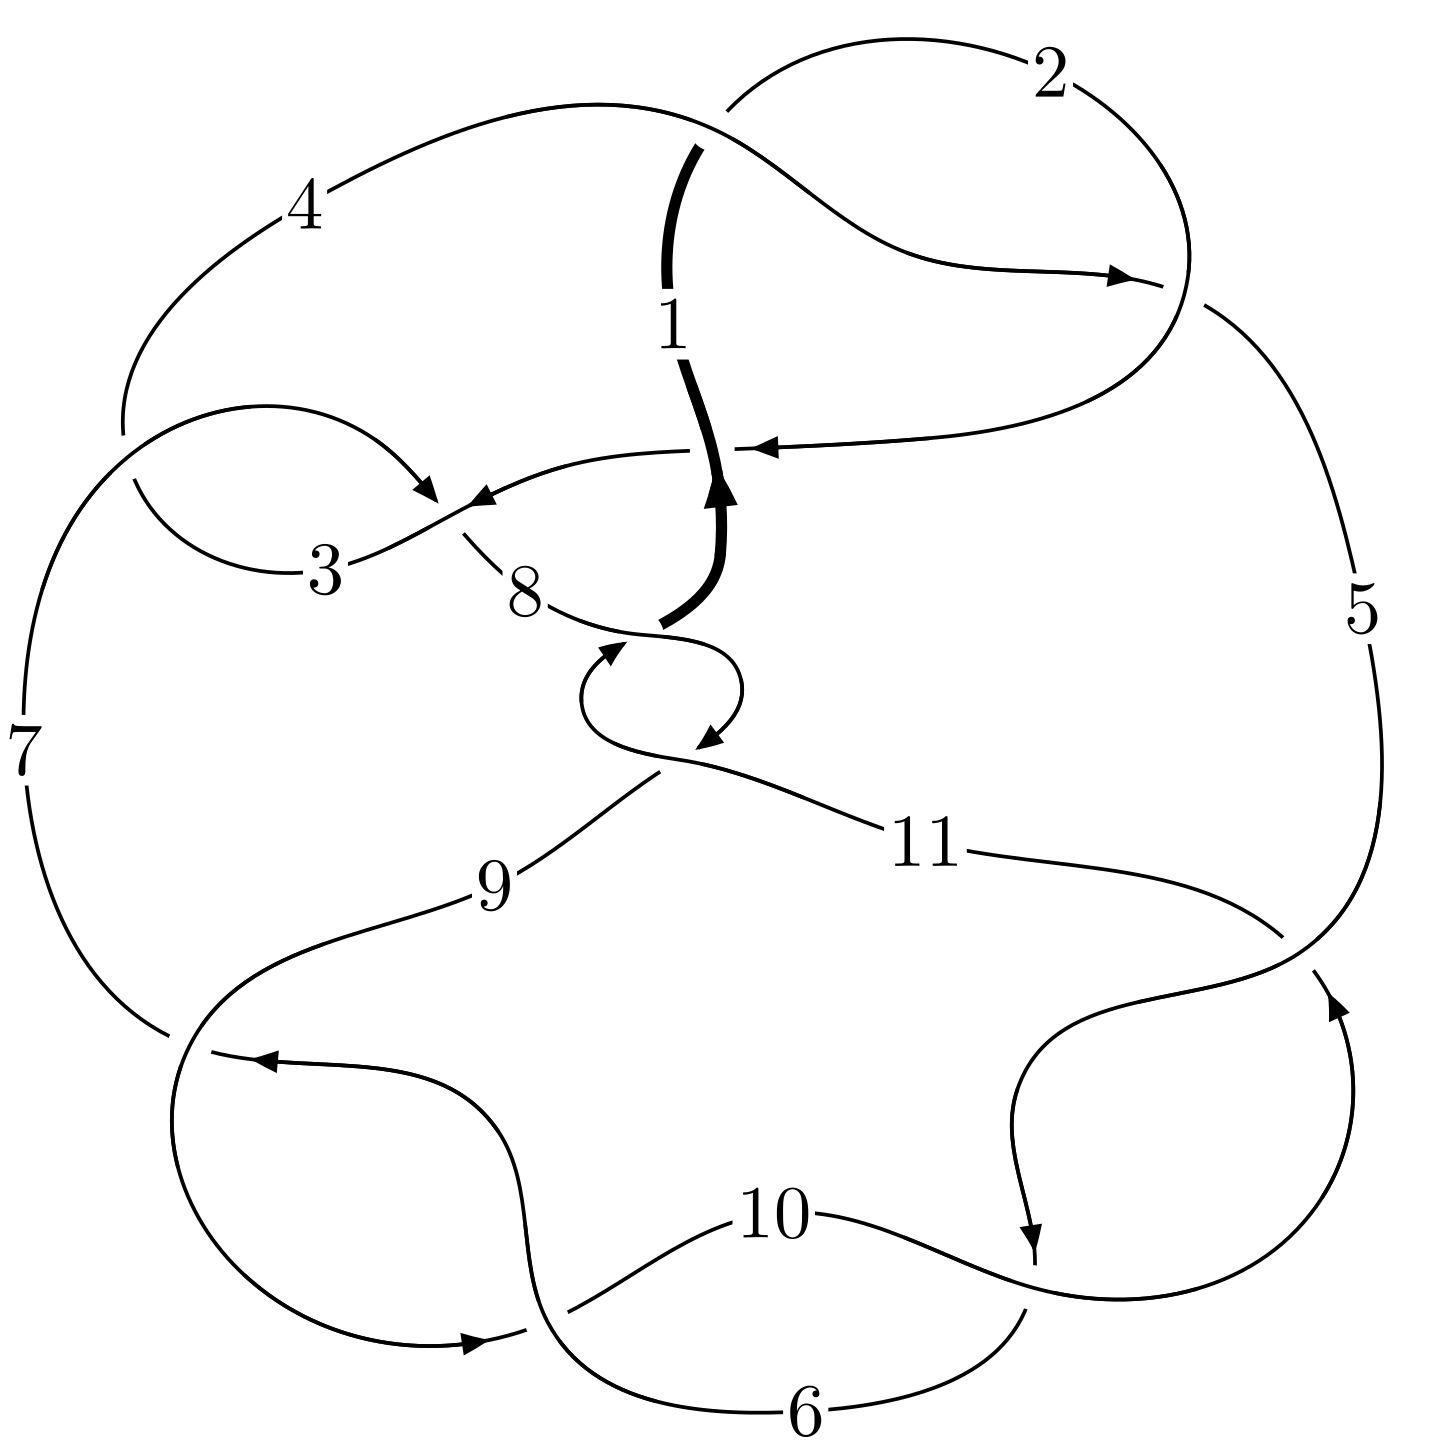
\includegraphics[width=112pt]{../../../GIT/diagram.site/Diagrams/png/294_11a_45.png}\\
\ \ \ A knot diagram\footnotemark}&
\allowdisplaybreaks
\textbf{Linearized knot diagam} \\
\cline{2-2}
 &
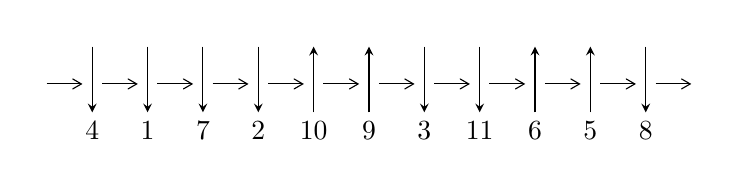
\begin{tikzpicture}[x=20pt, y=17pt]
	% nodes
	\node (C0) at (0, 0) {};
	\node (C1) at (1, 0) {};
	\node (C1U) at (1, +1) {};
	\node (C1D) at (1, -1) {4};

	\node (C2) at (2, 0) {};
	\node (C2U) at (2, +1) {};
	\node (C2D) at (2, -1) {1};

	\node (C3) at (3, 0) {};
	\node (C3U) at (3, +1) {};
	\node (C3D) at (3, -1) {7};

	\node (C4) at (4, 0) {};
	\node (C4U) at (4, +1) {};
	\node (C4D) at (4, -1) {2};

	\node (C5) at (5, 0) {};
	\node (C5U) at (5, +1) {};
	\node (C5D) at (5, -1) {10};

	\node (C6) at (6, 0) {};
	\node (C6U) at (6, +1) {};
	\node (C6D) at (6, -1) {9};

	\node (C7) at (7, 0) {};
	\node (C7U) at (7, +1) {};
	\node (C7D) at (7, -1) {3};

	\node (C8) at (8, 0) {};
	\node (C8U) at (8, +1) {};
	\node (C8D) at (8, -1) {11};

	\node (C9) at (9, 0) {};
	\node (C9U) at (9, +1) {};
	\node (C9D) at (9, -1) {6};

	\node (C10) at (10, 0) {};
	\node (C10U) at (10, +1) {};
	\node (C10D) at (10, -1) {5};

	\node (C11) at (11, 0) {};
	\node (C11U) at (11, +1) {};
	\node (C11D) at (11, -1) {8};
	\node (C12) at (12, 0) {};

	% arrows
	\draw[->,>={angle 60}]
	(C0) edge (C1) (C1) edge (C2) (C2) edge (C3) (C3) edge (C4) (C4) edge (C5) (C5) edge (C6) (C6) edge (C7) (C7) edge (C8) (C8) edge (C9) (C9) edge (C10) (C10) edge (C11) (C11) edge (C12) ;	\draw[->,>=stealth]
	(C1U) edge (C1D) (C2U) edge (C2D) (C3U) edge (C3D) (C4U) edge (C4D) (C5D) edge (C5U) (C6D) edge (C6U) (C7U) edge (C7D) (C8U) edge (C8D) (C9D) edge (C9U) (C10D) edge (C10U) (C11U) edge (C11D) ;
	\end{tikzpicture} \\
\hhline{~~} \\& 
\textbf{Solving Sequence} \\ \cline{2-2} 
 &
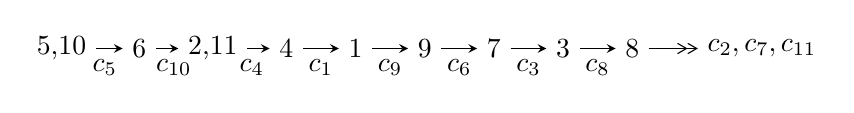
\begin{tikzpicture}[x=25pt, y=7pt]
	% node
	\node (A0) at (-1/8, 0) {5,10};
	\node (A1) at (1, 0) {6};
	\node (A2) at (33/16, 0) {2,11};
	\node (A3) at (25/8, 0) {4};
	\node (A4) at (33/8, 0) {1};
	\node (A5) at (41/8, 0) {9};
	\node (A6) at (49/8, 0) {7};
	\node (A7) at (57/8, 0) {3};
	\node (A8) at (65/8, 0) {8};
	\node (C1) at (1/2, -1) {$c_{5}$};
	\node (C2) at (3/2, -1) {$c_{10}$};
	\node (C3) at (21/8, -1) {$c_{4}$};
	\node (C4) at (29/8, -1) {$c_{1}$};
	\node (C5) at (37/8, -1) {$c_{9}$};
	\node (C6) at (45/8, -1) {$c_{6}$};
	\node (C7) at (53/8, -1) {$c_{3}$};
	\node (C8) at (61/8, -1) {$c_{8}$};
	\node (A9) at (10, 0) {$c_{2},c_{7},c_{11}$};

	% edge
	\draw[->,>=stealth]	
	(A0) edge (A1) (A1) edge (A2) (A2) edge (A3) (A3) edge (A4) (A4) edge (A5) (A5) edge (A6) (A6) edge (A7) (A7) edge (A8) ;
	\draw[->>,>={angle 60}]	
	(A8) edge (A9);
\end{tikzpicture} \\ 

\end{tabular} \\

\footnotetext{
The image of knot diagram is generated by the software ``\textbf{Draw programme}" developed by Andrew Bartholomew(\url{http://www.layer8.co.uk/maths/draw/index.htm\#Running-draw}), where we modified some parts for our purpose(\url{https://github.com/CATsTAILs/LinksPainter}).
}\phantom \\ \newline 
\centering \textbf{Ideals for irreducible components\footnotemark of $X_{\text{par}}$} 
 
\begin{align*}
I^u_{1}&=\langle 
u^{43}+u^{42}+\cdots+b+1,\;- u^{46}-2 u^{45}+\cdots+a-2,\;u^{47}+2 u^{46}+\cdots+4 u+1\rangle \\
I^u_{2}&=\langle 
b+1,\;- u^3- u^2+a-3 u,\;u^4+u^3+3 u^2+2 u+1\rangle \\
\\
\end{align*}
\raggedright * 2 irreducible components of $\dim_{\mathbb{C}}=0$, with total 51 representations.\\
\footnotetext{All coefficients of polynomials are rational numbers. But the coefficients are sometimes approximated in decimal forms when there is not enough margin.}
\newpage
\renewcommand{\arraystretch}{1}
\centering \section*{I. $I^u_{1}= \langle u^{43}+u^{42}+\cdots+b+1,\;- u^{46}-2 u^{45}+\cdots+a-2,\;u^{47}+2 u^{46}+\cdots+4 u+1 \rangle$}
\flushleft \textbf{(i) Arc colorings}\\
\begin{tabular}{m{7pt} m{180pt} m{7pt} m{180pt} }
\flushright $a_{5}=$&$\begin{pmatrix}1\\0\end{pmatrix}$ \\
\flushright $a_{10}=$&$\begin{pmatrix}0\\u\end{pmatrix}$ \\
\flushright $a_{6}=$&$\begin{pmatrix}1\\- u^2\end{pmatrix}$ \\
\flushright $a_{2}=$&$\begin{pmatrix}u^{46}+2 u^{45}+\cdots+u+2\\- u^{43}- u^{42}+\cdots-9 u^3-1\end{pmatrix}$ \\
\flushright $a_{11}=$&$\begin{pmatrix}u\\u\end{pmatrix}$ \\
\flushright $a_{4}=$&$\begin{pmatrix}u^{46}+2 u^{45}+\cdots- u+2\\- u^{43}- u^{42}+\cdots- u-1\end{pmatrix}$ \\
\flushright $a_{1}=$&$\begin{pmatrix}u^9+4 u^7+3 u^5-2 u^3+u\\u^9+5 u^7+7 u^5+2 u^3+u\end{pmatrix}$ \\
\flushright $a_{9}=$&$\begin{pmatrix}- u\\u^3+u\end{pmatrix}$ \\
\flushright $a_{7}=$&$\begin{pmatrix}u^2+1\\- u^4-2 u^2\end{pmatrix}$ \\
\flushright $a_{3}=$&$\begin{pmatrix}u^{46}+2 u^{45}+\cdots+3 u+3\\u^{44}- u^{43}+\cdots+u^2-1\end{pmatrix}$ \\
\flushright $a_{8}=$&$\begin{pmatrix}u^5+2 u^3- u\\u^5+3 u^3+u\end{pmatrix}$\\ \flushright $a_{8}=$&$\begin{pmatrix}u^5+2 u^3- u\\u^5+3 u^3+u\end{pmatrix}$\\&\end{tabular}
\flushleft \textbf{(ii) Obstruction class $= -1$}\\~\\
\flushleft \textbf{(iii) Cusp Shapes $= u^{46}+2 u^{45}+\cdots-7 u-9$}\\~\\
\newpage\renewcommand{\arraystretch}{1}
\flushleft \textbf{(iv) u-Polynomials at the component}\newline \\
\begin{tabular}{m{50pt}|m{274pt}}
Crossings & \hspace{64pt}u-Polynomials at each crossing \\
\hline $$\begin{aligned}c_{1},c_{4}\end{aligned}$$&$\begin{aligned}
&u^{47}-5 u^{46}+\cdots-8 u+1
\end{aligned}$\\
\hline $$\begin{aligned}c_{2}\end{aligned}$$&$\begin{aligned}
&u^{47}+21 u^{46}+\cdots-6 u+1
\end{aligned}$\\
\hline $$\begin{aligned}c_{3},c_{7}\end{aligned}$$&$\begin{aligned}
&u^{47}+u^{46}+\cdots+40 u+16
\end{aligned}$\\
\hline $$\begin{aligned}c_{5},c_{6},c_{9}\\c_{10}\end{aligned}$$&$\begin{aligned}
&u^{47}+2 u^{46}+\cdots+4 u+1
\end{aligned}$\\
\hline $$\begin{aligned}c_{8},c_{11}\end{aligned}$$&$\begin{aligned}
&u^{47}-8 u^{46}+\cdots+616 u-49
\end{aligned}$\\
\hline
\end{tabular}\\~\\
\newpage\renewcommand{\arraystretch}{1}
\flushleft \textbf{(v) Riley Polynomials at the component}\newline \\
\begin{tabular}{m{50pt}|m{274pt}}
Crossings & \hspace{64pt}Riley Polynomials at each crossing \\
\hline $$\begin{aligned}c_{1},c_{4}\end{aligned}$$&$\begin{aligned}
&y^{47}-21 y^{46}+\cdots-6 y-1
\end{aligned}$\\
\hline $$\begin{aligned}c_{2}\end{aligned}$$&$\begin{aligned}
&y^{47}+15 y^{46}+\cdots-262 y-1
\end{aligned}$\\
\hline $$\begin{aligned}c_{3},c_{7}\end{aligned}$$&$\begin{aligned}
&y^{47}+27 y^{46}+\cdots-3264 y-256
\end{aligned}$\\
\hline $$\begin{aligned}c_{5},c_{6},c_{9}\\c_{10}\end{aligned}$$&$\begin{aligned}
&y^{47}+52 y^{46}+\cdots+12 y-1
\end{aligned}$\\
\hline $$\begin{aligned}c_{8},c_{11}\end{aligned}$$&$\begin{aligned}
&y^{47}+32 y^{46}+\cdots+287140 y-2401
\end{aligned}$\\
\hline
\end{tabular}\\~\\
\newpage\flushleft \textbf{(vi) Complex Volumes and Cusp Shapes}
$$\begin{array}{c|c|c}  
\text{Solutions to }I^u_{1}& \I (\text{vol} + \sqrt{-1}CS) & \text{Cusp shape}\\
 \hline 
\begin{aligned}
u &= -0.604283 + 0.592983 I \\
a &= \phantom{-}1.47187 - 1.86934 I \\
b &= \phantom{-}1.126700 + 0.685229 I\end{aligned}
 & \phantom{-}4.37990 - 10.31740 I & -1.65034 + 8.68510 I \\ \hline\begin{aligned}
u &= -0.604283 - 0.592983 I \\
a &= \phantom{-}1.47187 + 1.86934 I \\
b &= \phantom{-}1.126700 - 0.685229 I\end{aligned}
 & \phantom{-}4.37990 + 10.31740 I & -1.65034 - 8.68510 I \\ \hline\begin{aligned}
u &= \phantom{-}0.232115 + 0.798027 I \\
a &= \phantom{-}2.24071 + 0.38222 I \\
b &= \phantom{-}0.974632 - 0.559034 I\end{aligned}
 & -1.04927 + 4.94975 I & -5.93011 - 7.21371 I \\ \hline\begin{aligned}
u &= \phantom{-}0.232115 - 0.798027 I \\
a &= \phantom{-}2.24071 - 0.38222 I \\
b &= \phantom{-}0.974632 + 0.559034 I\end{aligned}
 & -1.04927 - 4.94975 I & -5.93011 + 7.21371 I \\ \hline\begin{aligned}
u &= -0.610300 + 0.553965 I \\
a &= -0.902531 - 0.046325 I \\
b &= \phantom{-}0.490595 - 0.918525 I\end{aligned}
 & \phantom{-}6.31726 - 4.42879 I & \phantom{-}1.23708 + 4.26556 I \\ \hline\begin{aligned}
u &= -0.610300 - 0.553965 I \\
a &= -0.902531 + 0.046325 I \\
b &= \phantom{-}0.490595 + 0.918525 I\end{aligned}
 & \phantom{-}6.31726 + 4.42879 I & \phantom{-}1.23708 - 4.26556 I \\ \hline\begin{aligned}
u &= \phantom{-}0.564268 + 0.532900 I \\
a &= -0.60777 - 2.13982 I \\
b &= -0.886230 + 0.571745 I\end{aligned}
 & \phantom{-}1.15387 + 4.21075 I & -2.42283 - 6.46620 I \\ \hline\begin{aligned}
u &= \phantom{-}0.564268 - 0.532900 I \\
a &= -0.60777 + 2.13982 I \\
b &= -0.886230 - 0.571745 I\end{aligned}
 & \phantom{-}1.15387 - 4.21075 I & -2.42283 + 6.46620 I \\ \hline\begin{aligned}
u &= \phantom{-}0.368403 + 0.677743 I \\
a &= \phantom{-}0.723270 + 1.043890 I \\
b &= \phantom{-}0.725690 + 0.454437 I\end{aligned}
 & -0.121886 + 0.686906 I & -2.62923 - 1.30814 I \\ \hline\begin{aligned}
u &= \phantom{-}0.368403 - 0.677743 I \\
a &= \phantom{-}0.723270 - 1.043890 I \\
b &= \phantom{-}0.725690 - 0.454437 I\end{aligned}
 & -0.121886 - 0.686906 I & -2.62923 + 1.30814 I\\
 \hline 
 \end{array}$$\newpage$$\begin{array}{c|c|c}  
\text{Solutions to }I^u_{1}& \I (\text{vol} + \sqrt{-1}CS) & \text{Cusp shape}\\
 \hline 
\begin{aligned}
u &= -0.631315 + 0.431371 I \\
a &= \phantom{-}0.384246 - 0.958542 I \\
b &= \phantom{-}0.543018 + 0.899712 I\end{aligned}
 & \phantom{-}6.67942 + 0.21804 I & \phantom{-}2.26501 + 2.20975 I \\ \hline\begin{aligned}
u &= -0.631315 - 0.431371 I \\
a &= \phantom{-}0.384246 + 0.958542 I \\
b &= \phantom{-}0.543018 - 0.899712 I\end{aligned}
 & \phantom{-}6.67942 - 0.21804 I & \phantom{-}2.26501 - 2.20975 I \\ \hline\begin{aligned}
u &= -0.641272 + 0.383119 I \\
a &= \phantom{-}0.022026 + 0.485329 I \\
b &= \phantom{-}1.094550 - 0.696965 I\end{aligned}
 & \phantom{-}4.99878 + 6.09831 I & \phantom{-}0.10454 - 2.74650 I \\ \hline\begin{aligned}
u &= -0.641272 - 0.383119 I \\
a &= \phantom{-}0.022026 - 0.485329 I \\
b &= \phantom{-}1.094550 + 0.696965 I\end{aligned}
 & \phantom{-}4.99878 - 6.09831 I & \phantom{-}0.10454 + 2.74650 I \\ \hline\begin{aligned}
u &= -0.536843 + 0.494469 I \\
a &= -0.97848 + 1.17374 I \\
b &= -1.286310 + 0.037305 I\end{aligned}
 & -0.20145 - 1.85701 I & -0.50975 + 4.37782 I \\ \hline\begin{aligned}
u &= -0.536843 - 0.494469 I \\
a &= -0.97848 - 1.17374 I \\
b &= -1.286310 - 0.037305 I\end{aligned}
 & -0.20145 + 1.85701 I & -0.50975 - 4.37782 I \\ \hline\begin{aligned}
u &= \phantom{-}0.565661 + 0.444526 I \\
a &= \phantom{-}0.741523 + 0.717629 I \\
b &= -0.806231 - 0.561068 I\end{aligned}
 & \phantom{-}1.41432 - 0.32518 I & -1.284718 - 0.498489 I \\ \hline\begin{aligned}
u &= \phantom{-}0.565661 - 0.444526 I \\
a &= \phantom{-}0.741523 - 0.717629 I \\
b &= -0.806231 + 0.561068 I\end{aligned}
 & \phantom{-}1.41432 + 0.32518 I & -1.284718 + 0.498489 I \\ \hline\begin{aligned}
u &= -0.073145 + 0.598544 I \\
a &= -2.60222 + 1.37444 I \\
b &= -1.034680 - 0.259393 I\end{aligned}
 & -2.92920 - 0.94552 I & -11.86909 + 0.58583 I \\ \hline\begin{aligned}
u &= -0.073145 - 0.598544 I \\
a &= -2.60222 - 1.37444 I \\
b &= -1.034680 + 0.259393 I\end{aligned}
 & -2.92920 + 0.94552 I & -11.86909 - 0.58583 I\\
 \hline 
 \end{array}$$\newpage$$\begin{array}{c|c|c}  
\text{Solutions to }I^u_{1}& \I (\text{vol} + \sqrt{-1}CS) & \text{Cusp shape}\\
 \hline 
\begin{aligned}
u &= \phantom{-}0.284667 + 0.487292 I \\
a &= \phantom{-}0.588067 + 0.203086 I \\
b &= \phantom{-}0.141384 + 0.220781 I\end{aligned}
 & -0.038903 + 1.106530 I & -0.72417 - 6.07516 I \\ \hline\begin{aligned}
u &= \phantom{-}0.284667 - 0.487292 I \\
a &= \phantom{-}0.588067 - 0.203086 I \\
b &= \phantom{-}0.141384 - 0.220781 I\end{aligned}
 & -0.038903 - 1.106530 I & -0.72417 + 6.07516 I \\ \hline\begin{aligned}
u &= -0.15656 + 1.43102 I \\
a &= \phantom{-}0.964258 - 0.136228 I \\
b &= \phantom{-}1.042580 - 0.719852 I\end{aligned}
 & -0.77593 + 3.28450 I & \phantom{-0.000000 } 0 \\ \hline\begin{aligned}
u &= -0.15656 - 1.43102 I \\
a &= \phantom{-}0.964258 + 0.136228 I \\
b &= \phantom{-}1.042580 + 0.719852 I\end{aligned}
 & -0.77593 - 3.28450 I & \phantom{-0.000000 } 0 \\ \hline\begin{aligned}
u &= \phantom{-}0.534809 + 0.072952 I \\
a &= \phantom{-}0.267834 + 0.634733 I \\
b &= \phantom{-}0.841064 - 0.586379 I\end{aligned}
 & \phantom{-}1.73762 + 2.33285 I & \phantom{-}1.63431 - 3.88919 I \\ \hline\begin{aligned}
u &= \phantom{-}0.534809 - 0.072952 I \\
a &= \phantom{-}0.267834 - 0.634733 I \\
b &= \phantom{-}0.841064 + 0.586379 I\end{aligned}
 & \phantom{-}1.73762 - 2.33285 I & \phantom{-}1.63431 + 3.88919 I \\ \hline\begin{aligned}
u &= -0.17342 + 1.46958 I \\
a &= \phantom{-}0.892690 - 0.159044 I \\
b &= \phantom{-}0.614156 + 0.885412 I\end{aligned}
 & \phantom{-}0.53093 - 2.62820 I & \phantom{-0.000000 } 0 \\ \hline\begin{aligned}
u &= -0.17342 - 1.46958 I \\
a &= \phantom{-}0.892690 + 0.159044 I \\
b &= \phantom{-}0.614156 - 0.885412 I\end{aligned}
 & \phantom{-}0.53093 + 2.62820 I & \phantom{-0.000000 } 0 \\ \hline\begin{aligned}
u &= \phantom{-}0.14450 + 1.50474 I \\
a &= \phantom{-}0.086605 + 0.128202 I \\
b &= -0.704621 - 0.592796 I\end{aligned}
 & -4.99092 + 2.12497 I & \phantom{-0.000000 } 0 \\ \hline\begin{aligned}
u &= \phantom{-}0.14450 - 1.50474 I \\
a &= \phantom{-}0.086605 - 0.128202 I \\
b &= -0.704621 + 0.592796 I\end{aligned}
 & -4.99092 - 2.12497 I & \phantom{-0.000000 } 0\\
 \hline 
 \end{array}$$\newpage$$\begin{array}{c|c|c}  
\text{Solutions to }I^u_{1}& \I (\text{vol} + \sqrt{-1}CS) & \text{Cusp shape}\\
 \hline 
\begin{aligned}
u &= -0.14983 + 1.52897 I \\
a &= -2.18209 + 0.88257 I \\
b &= -1.313780 + 0.094691 I\end{aligned}
 & -6.93429 - 4.28271 I & \phantom{-0.000000 } 0 \\ \hline\begin{aligned}
u &= -0.14983 - 1.52897 I \\
a &= -2.18209 - 0.88257 I \\
b &= -1.313780 - 0.094691 I\end{aligned}
 & -6.93429 + 4.28271 I & \phantom{-0.000000 } 0 \\ \hline\begin{aligned}
u &= \phantom{-}0.04949 + 1.54079 I \\
a &= \phantom{-}0.359833 + 0.420302 I \\
b &= \phantom{-}0.022840 + 0.536346 I\end{aligned}
 & -6.95405 + 2.13733 I & \phantom{-0.000000 } 0 \\ \hline\begin{aligned}
u &= \phantom{-}0.04949 - 1.54079 I \\
a &= \phantom{-}0.359833 - 0.420302 I \\
b &= \phantom{-}0.022840 - 0.536346 I\end{aligned}
 & -6.95405 - 2.13733 I & \phantom{-0.000000 } 0 \\ \hline\begin{aligned}
u &= \phantom{-}0.16493 + 1.53761 I \\
a &= -1.47288 - 1.40203 I \\
b &= -0.945052 + 0.589157 I\end{aligned}
 & -5.72542 + 6.83119 I & \phantom{-0.000000 } 0 \\ \hline\begin{aligned}
u &= \phantom{-}0.16493 - 1.53761 I \\
a &= -1.47288 + 1.40203 I \\
b &= -0.945052 - 0.589157 I\end{aligned}
 & -5.72542 - 6.83119 I & \phantom{-0.000000 } 0 \\ \hline\begin{aligned}
u &= -0.18579 + 1.54140 I \\
a &= -0.364549 - 0.727740 I \\
b &= \phantom{-}0.443402 - 0.937849 I\end{aligned}
 & -0.62096 - 7.31850 I & \phantom{-0.000000 } 0 \\ \hline\begin{aligned}
u &= -0.18579 - 1.54140 I \\
a &= -0.364549 + 0.727740 I \\
b &= \phantom{-}0.443402 + 0.937849 I\end{aligned}
 & -0.62096 + 7.31850 I & \phantom{-0.000000 } 0 \\ \hline\begin{aligned}
u &= -0.01255 + 1.55908 I \\
a &= -2.70333 + 0.61165 I \\
b &= -1.133330 - 0.334796 I\end{aligned}
 & -10.25720 - 1.20723 I & \phantom{-0.000000 } 0 \\ \hline\begin{aligned}
u &= -0.01255 - 1.55908 I \\
a &= -2.70333 - 0.61165 I \\
b &= -1.133330 + 0.334796 I\end{aligned}
 & -10.25720 + 1.20723 I & \phantom{-0.000000 } 0\\
 \hline 
 \end{array}$$\newpage$$\begin{array}{c|c|c}  
\text{Solutions to }I^u_{1}& \I (\text{vol} + \sqrt{-1}CS) & \text{Cusp shape}\\
 \hline 
\begin{aligned}
u &= -0.18591 + 1.55945 I \\
a &= \phantom{-}2.26208 - 1.08076 I \\
b &= \phantom{-}1.152470 + 0.673628 I\end{aligned}
 & -2.78197 - 13.21230 I & \phantom{-0.000000 } 0 \\ \hline\begin{aligned}
u &= -0.18591 - 1.55945 I \\
a &= \phantom{-}2.26208 + 1.08076 I \\
b &= \phantom{-}1.152470 - 0.673628 I\end{aligned}
 & -2.78197 + 13.21230 I & \phantom{-0.000000 } 0 \\ \hline\begin{aligned}
u &= \phantom{-}0.10845 + 1.58073 I \\
a &= \phantom{-}1.54084 + 0.82842 I \\
b &= \phantom{-}0.782367 + 0.305537 I\end{aligned}
 & -7.73076 + 2.45052 I & \phantom{-0.000000 } 0 \\ \hline\begin{aligned}
u &= \phantom{-}0.10845 - 1.58073 I \\
a &= \phantom{-}1.54084 - 0.82842 I \\
b &= \phantom{-}0.782367 - 0.305537 I\end{aligned}
 & -7.73076 - 2.45052 I & \phantom{-0.000000 } 0 \\ \hline\begin{aligned}
u &= \phantom{-}0.04923 + 1.60296 I \\
a &= \phantom{-}2.55612 - 0.07351 I \\
b &= \phantom{-}1.041330 - 0.500879 I\end{aligned}
 & -9.19770 + 5.90087 I & \phantom{-0.000000 } 0 \\ \hline\begin{aligned}
u &= \phantom{-}0.04923 - 1.60296 I \\
a &= \phantom{-}2.55612 + 0.07351 I \\
b &= \phantom{-}1.041330 + 0.500879 I\end{aligned}
 & -9.19770 - 5.90087 I & \phantom{-0.000000 } 0 \\ \hline\begin{aligned}
u &= -0.210582\phantom{ +0.000000I} \\
a &= \phantom{-}2.42377\phantom{ +0.000000I} \\
b &= -0.853085\phantom{ +0.000000I}\end{aligned}
 & -1.24674\phantom{ +0.000000I} & -7.85810\phantom{ +0.000000I}\\
 \hline 
 \end{array}$$\newpage\newpage\renewcommand{\arraystretch}{1}
\centering \section*{II. $I^u_{2}= \langle b+1,\;- u^3- u^2+a-3 u,\;u^4+u^3+3 u^2+2 u+1 \rangle$}
\flushleft \textbf{(i) Arc colorings}\\
\begin{tabular}{m{7pt} m{180pt} m{7pt} m{180pt} }
\flushright $a_{5}=$&$\begin{pmatrix}1\\0\end{pmatrix}$ \\
\flushright $a_{10}=$&$\begin{pmatrix}0\\u\end{pmatrix}$ \\
\flushright $a_{6}=$&$\begin{pmatrix}1\\- u^2\end{pmatrix}$ \\
\flushright $a_{2}=$&$\begin{pmatrix}u^3+u^2+3 u\\-1\end{pmatrix}$ \\
\flushright $a_{11}=$&$\begin{pmatrix}u\\u\end{pmatrix}$ \\
\flushright $a_{4}=$&$\begin{pmatrix}u^3+u^2+3 u+1\\-1\end{pmatrix}$ \\
\flushright $a_{1}=$&$\begin{pmatrix}-1\\0\end{pmatrix}$ \\
\flushright $a_{9}=$&$\begin{pmatrix}- u\\u^3+u\end{pmatrix}$ \\
\flushright $a_{7}=$&$\begin{pmatrix}u^2+1\\u^3+u^2+2 u+1\end{pmatrix}$ \\
\flushright $a_{3}=$&$\begin{pmatrix}u^3+u^2+3 u+1\\-1\end{pmatrix}$ \\
\flushright $a_{8}=$&$\begin{pmatrix}u^2+1\\u^3+u^2+2 u+1\end{pmatrix}$\\ \flushright $a_{8}=$&$\begin{pmatrix}u^2+1\\u^3+u^2+2 u+1\end{pmatrix}$\\&\end{tabular}
\flushleft \textbf{(ii) Obstruction class $= 1$}\\~\\
\flushleft \textbf{(iii) Cusp Shapes $= 3 u^3+3 u^2+10 u-4$}\\~\\
\newpage\renewcommand{\arraystretch}{1}
\flushleft \textbf{(iv) u-Polynomials at the component}\newline \\
\begin{tabular}{m{50pt}|m{274pt}}
Crossings & \hspace{64pt}u-Polynomials at each crossing \\
\hline $$\begin{aligned}c_{1}\end{aligned}$$&$\begin{aligned}
&(u-1)^4
\end{aligned}$\\
\hline $$\begin{aligned}c_{2},c_{4}\end{aligned}$$&$\begin{aligned}
&(u+1)^4
\end{aligned}$\\
\hline $$\begin{aligned}c_{3},c_{7}\end{aligned}$$&$\begin{aligned}
&u^4
\end{aligned}$\\
\hline $$\begin{aligned}c_{5},c_{6}\end{aligned}$$&$\begin{aligned}
&u^4+u^3+3 u^2+2 u+1
\end{aligned}$\\
\hline $$\begin{aligned}c_{8}\end{aligned}$$&$\begin{aligned}
&u^4+u^3+u^2+1
\end{aligned}$\\
\hline $$\begin{aligned}c_{9},c_{10}\end{aligned}$$&$\begin{aligned}
&u^4- u^3+3 u^2-2 u+1
\end{aligned}$\\
\hline $$\begin{aligned}c_{11}\end{aligned}$$&$\begin{aligned}
&u^4- u^3+u^2+1
\end{aligned}$\\
\hline
\end{tabular}\\~\\
\newpage\renewcommand{\arraystretch}{1}
\flushleft \textbf{(v) Riley Polynomials at the component}\newline \\
\begin{tabular}{m{50pt}|m{274pt}}
Crossings & \hspace{64pt}Riley Polynomials at each crossing \\
\hline $$\begin{aligned}c_{1},c_{2},c_{4}\end{aligned}$$&$\begin{aligned}
&(y-1)^4
\end{aligned}$\\
\hline $$\begin{aligned}c_{3},c_{7}\end{aligned}$$&$\begin{aligned}
&y^4
\end{aligned}$\\
\hline $$\begin{aligned}c_{5},c_{6},c_{9}\\c_{10}\end{aligned}$$&$\begin{aligned}
&y^4+5 y^3+7 y^2+2 y+1
\end{aligned}$\\
\hline $$\begin{aligned}c_{8},c_{11}\end{aligned}$$&$\begin{aligned}
&y^4+y^3+3 y^2+2 y+1
\end{aligned}$\\
\hline
\end{tabular}\\~\\
\newpage\flushleft \textbf{(vi) Complex Volumes and Cusp Shapes}
$$\begin{array}{c|c|c}  
\text{Solutions to }I^u_{2}& \I (\text{vol} + \sqrt{-1}CS) & \text{Cusp shape}\\
 \hline 
\begin{aligned}
u &= -0.395123 + 0.506844 I \\
a &= -1.04332 + 1.22719 I \\
b &= -1.00000\phantom{ +0.000000I}\end{aligned}
 & -1.43393 - 1.41510 I & -7.52507 + 4.18840 I \\ \hline\begin{aligned}
u &= -0.395123 - 0.506844 I \\
a &= -1.04332 - 1.22719 I \\
b &= -1.00000\phantom{ +0.000000I}\end{aligned}
 & -1.43393 + 1.41510 I & -7.52507 - 4.18840 I \\ \hline\begin{aligned}
u &= -0.10488 + 1.55249 I \\
a &= -1.95668 + 0.64120 I \\
b &= -1.00000\phantom{ +0.000000I}\end{aligned}
 & -8.43568 - 3.16396 I & -9.97493 + 3.47609 I \\ \hline\begin{aligned}
u &= -0.10488 - 1.55249 I \\
a &= -1.95668 - 0.64120 I \\
b &= -1.00000\phantom{ +0.000000I}\end{aligned}
 & -8.43568 + 3.16396 I & -9.97493 - 3.47609 I\\
 \hline 
 \end{array}$$\newpage
\newpage\renewcommand{\arraystretch}{1}
\centering \section*{ III. u-Polynomials}
\begin{tabular}{m{50pt}|m{274pt}}
Crossings & \hspace{64pt}u-Polynomials at each crossing \\
\hline $$\begin{aligned}c_{1}\end{aligned}$$&$\begin{aligned}
&((u-1)^4)(u^{47}-5 u^{46}+\cdots-8 u+1)
\end{aligned}$\\
\hline $$\begin{aligned}c_{2}\end{aligned}$$&$\begin{aligned}
&((u+1)^4)(u^{47}+21 u^{46}+\cdots-6 u+1)
\end{aligned}$\\
\hline $$\begin{aligned}c_{3},c_{7}\end{aligned}$$&$\begin{aligned}
&u^4(u^{47}+u^{46}+\cdots+40 u+16)
\end{aligned}$\\
\hline $$\begin{aligned}c_{4}\end{aligned}$$&$\begin{aligned}
&((u+1)^4)(u^{47}-5 u^{46}+\cdots-8 u+1)
\end{aligned}$\\
\hline $$\begin{aligned}c_{5},c_{6}\end{aligned}$$&$\begin{aligned}
&(u^4+u^3+3 u^2+2 u+1)(u^{47}+2 u^{46}+\cdots+4 u+1)
\end{aligned}$\\
\hline $$\begin{aligned}c_{8}\end{aligned}$$&$\begin{aligned}
&(u^4+u^3+u^2+1)(u^{47}-8 u^{46}+\cdots+616 u-49)
\end{aligned}$\\
\hline $$\begin{aligned}c_{9},c_{10}\end{aligned}$$&$\begin{aligned}
&(u^4- u^3+3 u^2-2 u+1)(u^{47}+2 u^{46}+\cdots+4 u+1)
\end{aligned}$\\
\hline $$\begin{aligned}c_{11}\end{aligned}$$&$\begin{aligned}
&(u^4- u^3+u^2+1)(u^{47}-8 u^{46}+\cdots+616 u-49)
\end{aligned}$\\
\hline
\end{tabular}\newpage\renewcommand{\arraystretch}{1}
\centering \section*{ IV. Riley Polynomials}
\begin{tabular}{m{50pt}|m{274pt}}
Crossings & \hspace{64pt}Riley Polynomials at each crossing \\
\hline $$\begin{aligned}c_{1},c_{4}\end{aligned}$$&$\begin{aligned}
&((y-1)^4)(y^{47}-21 y^{46}+\cdots-6 y-1)
\end{aligned}$\\
\hline $$\begin{aligned}c_{2}\end{aligned}$$&$\begin{aligned}
&((y-1)^4)(y^{47}+15 y^{46}+\cdots-262 y-1)
\end{aligned}$\\
\hline $$\begin{aligned}c_{3},c_{7}\end{aligned}$$&$\begin{aligned}
&y^4(y^{47}+27 y^{46}+\cdots-3264 y-256)
\end{aligned}$\\
\hline $$\begin{aligned}c_{5},c_{6},c_{9}\\c_{10}\end{aligned}$$&$\begin{aligned}
&(y^4+5 y^3+7 y^2+2 y+1)(y^{47}+52 y^{46}+\cdots+12 y-1)
\end{aligned}$\\
\hline $$\begin{aligned}c_{8},c_{11}\end{aligned}$$&$\begin{aligned}
&(y^4+y^3+3 y^2+2 y+1)(y^{47}+32 y^{46}+\cdots+287140 y-2401)
\end{aligned}$\\
\hline
\end{tabular}
\vskip 2pc
\end{document}